\documentclass[a4paper]{article}
\usepackage[pdftex]{graphicx}
\usepackage[utf8]{inputenc}
\usepackage{enumerate}
\usepackage{amssymb}
\usepackage{icomma}
\usepackage{siunitx}
\sisetup{locale=DE} 
\usepackage{tikz}
\usepackage{href-ul}
\hypersetup{
	colorlinks=true,
	linkcolor=blue,
	urlcolor=blue}
\usepackage{geometry}
\geometry{a4paper, top=15mm, left=15mm, right=15mm, bottom=15mm,
	headsep=10mm, footskip=12mm}

\begin{document}
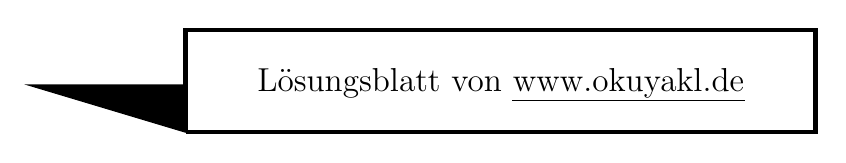
\begin{tikzpicture}(10,3)
	\draw[ultra thick](2,0) --(10,0) -- (10,1.3) --(2,1.3) -- (2,0);
	\draw[fill=black](2,0)-- (0,.6) -- (2,.6) -- (2,0);
	\node at (6,.6) {\large Lösungsblatt von \href{https://www.okuyakl.de}{www.okuyakl.de}};
\end{tikzpicture}
\vspace{0.5 cm}

\noindent{\bf Aufgabe 1.}\\


\renewcommand{\arraystretch}{1.8}
\begin{tabular}{|p{1.7 cm}|p{1.7 cm}|p{1.7 cm}|p{1.7 cm}|p{1.7 cm}|p{1.7 cm}|p{1.7 cm}|p{1.7 cm}|}
\hline
Stoff	& Holz & Blei & Wasser & Luft & Speiseöl & Gold & Aluminium \\
\hline 
Zustand & fest & fest & flüssig & gasförmig & flüssig & fest & fest \\
\hline
Beispiel & Bauklotz & Anglerblei & Flasche & Ballon & Flasche & Barren & Spitzer\\
\hline
Masse & $\SI{35}{\gram}$  & $\SI{5,0}{\gram}$  & $\SI{1,5}{\kilo\gram}$  & $\SI{5,2}{\gram}$  & $\SI{0,63}{\kilogram}$  & $\SI{12,4}{\kilogram}$  &$\SI{4,3}{\gram}$  \\
\hline
Volumen &$\SI{50}{\centi\meter^3}$  & $\SI{0,44}{\centi\meter^3}$  &$\SI{1,5}{\deci\meter^3}$  & $\SI{4,0}{\deci\meter^3}$  & $\SI{0,7}{\deci\meter^3 }$  &$\SI{0,64}{\deci\meter^3}$  & $\SI{1,6}{\centi\meter^3}$  \\
\hline
Dichte &$\SI{0,7}{\gram\over\centi\meter^3}$  &$\SI{11,3}{\gram\over\centi\meter^3}$  &$\SI{1,0}{\gram\over\centi\meter^3}$  &$\SI{1,3}{\gram\over \deci\meter^3}$  &$\SI{0,9}{\gram\over\centi\meter^3}$  &$\SI{19,3}{\gram\over\centi\meter^3}$  &$\SI{2,7}{\gram\over\centi\meter^3}$  \\
\hline
\end{tabular}
\vspace{0.5 cm}

\begin{tabular}{|p{1.4 cm}|p{1.4 cm}|p{1.5 cm}|p{1.8 cm}|p{1.7 cm}|p{2.0 cm}|p{2.1 cm}|p{1.7 cm}|}
\hline
Stoff	& Kork & Eisen & Styropor & Wasserstoff & Iridium & Quecksilber & Polyethylen \\
\hline
Zustand & fest & fest & fest & gasförmig & fest & flüssig & fest \\
\hline 
Beispiel & Korken & Schlüssel & Dämmplatte & Ballon & Urkilogramm & Thermometer & Spielwürfel\\
\hline
Masse &$\SI{1,9}{\gram}$  &$\SI{8,5}{\gram}$  & $\SI{150}{\gram}$  & $\SI{0,41}{\gram}$  & $\SI{1,0}{\kilogram}$  & $\SI{0,67}{\gram}$ & $\SI{3,1}{\gram}$\\
\hline
Volumen &$\SI{6,2}{\centi\meter^3}$  & $\SI{1,1}{\centi\meter^3}$  & $\SI{5,0}{\deci\meter^3}$  & $\SI{4,5}{\deci\meter^3}$  & $\SI{45}{\centi\meter^3}$  &$\SI{0,05}{\centi\meter^3}$  &$\SI{3,3}{\centi\meter^3}$  \\
\hline
Dichte &$\SI{0,3}{\gram\over\centi\meter^3}$  &$\SI{7,7}{\gram\over\centi\meter^3}$  &$\SI{0,03}{\gram\over\centi\meter^3}$  &$\SI{90}{\gram\over\meter^3}$  &$\SI{22,4}{\gram\over\centi\meter^3}$  &$\SI{13,5}{\gram\over\centi\meter^3}$  &$\SI{0,95}{\gram\over\centi\meter^3}$  \\
\hline
\end{tabular}
\vspace{0.5 cm}

\noindent{\bf Aufgabe 2.}\\
Leichtester Stoff: Wasserstoff; schwerster Stoff: Iridium
\vspace{0.5 cm}

\noindent{\bf Aufgabe 3.}\\
Die umgebende Luft ist spezifisch schwerer als der Wasserstoffballon, darum erfährt er eine Auftriebskraft
\vspace{0.5 cm}

\noindent{\bf Aufgabe 4. a)}\\
\renewcommand{\arraystretch}{2}
\begin{tabular}{|p{3 cm}|p{12.5 cm}|}
	\hline
	Schwimmt in & Stoff \\
	\hline
	Speiseöl & Holz, Kork, Styropor\\
	\hline
	Wasser	& Holz, Kork, Styropor, Polyethylen \\
	\hline
	Quecksilber & Holz, Kork, Styropor, Polyethylen, Blei, Eisen, Aluminium\\
	\hline
\end{tabular}
\vspace{0.5 cm}

\noindent{\bf Aufgabe 4. b)}\\
Polyethylen ist spezifisch schwerer als Speiseöl, aber leichter als Wasser
\vspace{0.5 cm}

\noindent{\bf Aufgabe 4. c)}\\ 
Gold, Iridium.

\begin{center}
	\includegraphics[width=7 cm]{../../viecher/endcomic.pdf}
	
	Hier geht es zurück zum \href{https://www.okuyakl.de/phys/p7dihL073/aa073.pdf}{Aufgabenblatt}
\end{center}



\end{document}

